\section{Exploración Inicial} \label{chapt:initial_exploration}

El objetivo de esta exploración es escoger los parámetros: dimensión del cromosoma (\textit{DIM}) y tamaño de población. Primero se varía la dimensión
del cromosoma y la población se mantiene fija a 100. Se ejecutará el algoritmo 15 veces por cada dimensión del cromosoma, y se cogerá el que 
tenga mejor resultado para la comparación. Los resultados de esta primera exploración se encuentran en la Tabla \ref{tab:fitness_variation}. 

\begin{table}[]
    \centering
    \begin{tabular}{||c|c|c|c|c|c||}
        \hline
        \textbf{Fichero Configuración} & \textbf{Generaciones} & \textbf{DIM} & \textbf{Mejor fitness} & \textbf{Evals. de f}\\ \hline
        Config 1   & 16    & 2   & -76.93    &  2340  \\ \hline
        Config 2   & 20    & 3   & -74.70    &  2900  \\ \hline
        Config 3   & 20    & 5   & -67.58    &  2900  \\ \hline
        Config 4   & 56    & 10  & -45.74    &  8567  \\ \hline
        Config 5   & 68    & 20  & 49.43     &  10494 \\ \hline
        Config 6   & 52    & 40  & 422.26    &  8133  \\ \hline
    \end{tabular}
    \caption{Resultados exploración inicial}
    \label{tab:fitness_variation}
\end{table}

\begin{figure}[]
	\centering	
	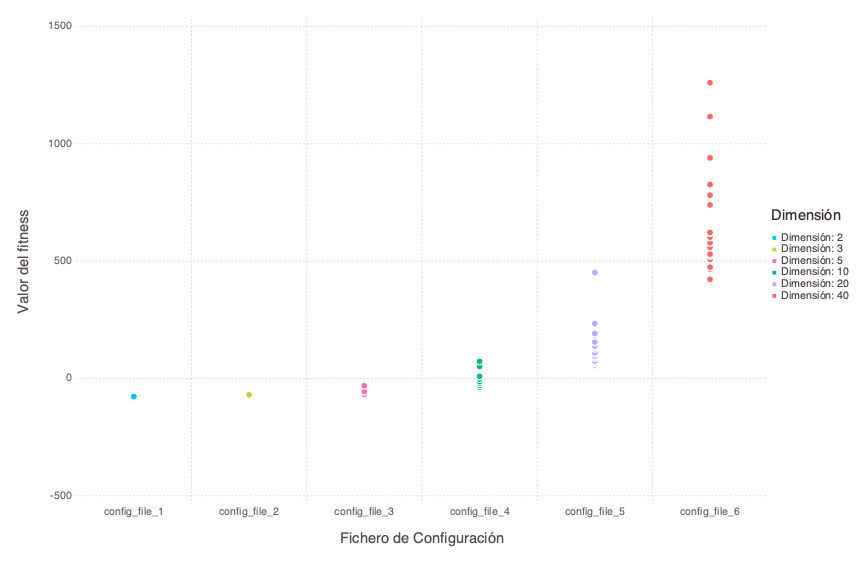
\includegraphics[scale=0.4]{figuras/config_file_1-6_Rastrigin_box_plots.png}
	\caption{ Variación del valor del fitness }
    \label{fig:box_plots}
\end{figure}

Para un tamaño de población 100 aparentemente la mejor dimensión es la 3. Sin embargo, mirando la Figura \ref{fig:box_plots} comprobamos
que la configuración 2 apenas ha explorado el espacio, mas ha alcanzado un óptimo local, al igual que de la 1 a la 3. Para
futuras explotaciones descartaremos estas configuraciones, ya que no aportan apenas información sobre el comportamiento del algoritmo.
Con la información extraída de estos experimentos no se puede concluir qué valores escoger para el tamaño de población ni para la
dimensión del cromosoma. En las siguientes secciones se le dará un enfoque diferente.
